% !TeX program = xelatex
\documentclass[UTF8,a4paper,11pt,fontset=windows]{ctexart}
\usepackage[left=18mm,right=18mm,top=16mm,bottom=17mm,headheight=14pt]{geometry}
\usepackage{amsmath,amssymb,array,booktabs,longtable,needspace,fancyhdr,xcolor,tikz}
\usepackage[hidelinks]{hyperref}
\setlength{\parindent}{0pt}\setlength{\parskip}{3pt}\linespread{1.1}
\setlength{\emergencystretch}{2em}\raggedbottom
\pagestyle{fancy}\fancyhf{}\renewcommand{\headrulewidth}{0pt}
\fancyfoot[C]{\small\PaperName\quad 第\thepage 页}
\newcommand{\R}{\mathbb R}
\newcommand{\blank}{\underline{\hspace{2.9cm}}}
\newcommand{\src}[1]{\par{\scriptsize\color{black!65}教材改编出处：#1。}\par}
\newcommand{\q}[2]{\par\Needspace{4\baselineskip}\textbf{#1.}\ #2}
\newcommand{\subq}[2]{\par\Needspace{2\baselineskip}（#1）#2}
\newcommand{\opts}[4]{\par\begin{tabular*}{\linewidth}{@{}p{.48\linewidth}@{\extracolsep{\fill}}p{.48\linewidth}@{}}A. #1&B. #2\\C. #3&D. #4\end{tabular*}\par}
\newcommand{\optsfour}[4]{\par\begin{tabular*}{\linewidth}{@{}p{.235\linewidth}@{\extracolsep{\fill}}p{.235\linewidth}p{.235\linewidth}p{.235\linewidth}@{}}A. #1&B. #2&C. #3&D. #4\end{tabular*}\par}
\newcommand{\parttitle}[1]{\par\Needspace{4\baselineskip}{\bfseries #1}\par}
\newcommand{\work}[1]{\par\vspace*{#1}}
\newcommand{\ans}[2]{\par\Needspace{4\baselineskip}\textbf{第#1题}\quad #2\par}
\newcommand{\readinggraph}{\begin{center}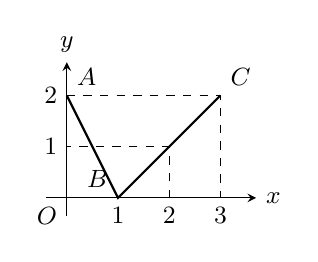
\begin{tikzpicture}[x=.65cm,y=.65cm,>=stealth,font=\small]
\draw[->](-.4,0)--(3.7,0)node[right]{$x$};\draw[->](0,-.35)--(0,2.65)node[above]{$y$};
\draw[thick](0,2)node[above right]{$A$}--(1,0)node[above left]{$B$}--(3,2)node[above right]{$C$};
\draw[dashed](0,2)--(3,2)--(3,0);\draw[dashed](2,0)--(2,1)--(0,1);
\node[below left]at(0,0){$O$};\foreach \x in {1,2,3}\node[below]at(\x,0){$\x$};
\foreach \y in {1,2}\node[left]at(0,\y){$\y$};\end{tikzpicture}\end{center}}
\renewcommand{\arraystretch}{1.2}

\newcommand{\PaperName}{A卷参考答案与评分}
\begin{document}
\begin{center}{\Large\bfseries 高一数学期中教材改编练习卷（A）}\\[2mm]参考答案、评分细则与教材出处\end{center}
单选、填空每题5分；多选全对6分，部分选对且无错项3分，含错项或未选0分。以下评分为本练习卷统一约定；解答题其他正确解法按相应步骤给分。
\parttitle{答案速查}\begin{center}\begin{tabular}{c|cccccccc}\toprule 题号&1&2&3&4&5&6&7&8\\答案&B&A&D&C&B&A&C&D\\\bottomrule\end{tabular}\par\smallskip\begin{tabular}{c|cccccc}\toprule 题号&9&10&11&12&13&14\\答案&AB&ABD&ABD&$(4,+\infty)$&$3$&$[4,+\infty)$\\\bottomrule\end{tabular}\end{center}
\parttitle{单项选择题解析}
\ans{1}{\textbf{B}。同时属于两个集合的元素为2、5，故交集为 $\{2,5\}$。}
\ans{2}{\textbf{A}。$x=1$ 能推出 $x^2=1$，反向不成立，反例为 $x=-1$。}
\ans{3}{\textbf{D}。否定全称命题时改为存在量词，范围不变，$>0$ 改为 $\le0$。}
\ans{4}{\textbf{C}。令 $t=x-1>0$，则原式为 $1+t+9/t\ge1+6=7$；等号在 $t=3$，即 $x=4$ 时取得。}
\ans{5}{\textbf{B}。A的第二个函数在 $x=-1$ 无定义；B两函数定义域均为 $\R$ 且对应关系相同；C对应关系不同；D第二个函数定义域为 $[0,+\infty)$。}
\ans{6}{\textbf{A}。须同时有 $x\le3$ 与 $x\ne1$，故定义域为 $(-\infty,1)\cup(1,3]$。}
\ans{7}{\textbf{C}。$f(2)=8$，由奇性得 $f(-2)=-f(2)=-8$。题设相容，取 $f(0)=0$ 并作奇延拓即可。}
\ans{8}{\textbf{D}。对称轴为 $x=a$。给定区间必须位于对称轴左侧（可含轴），故 $a\ge3$；$a=3$ 时仍严格递减。}
\parttitle{多项选择题与填空题解析}
\ans{9}{\textbf{AB}。A：正数取倒数后大小反向，正确。B：正数平方保序，正确。C：$a/b>1$，故错误。D：取 $c=0$ 时两边相等，故“任意实数c”下不成立。}
\ans{10}{\textbf{ABD}。$f(x)=(x-1)^2-1$，最小值为 $-1$；端点值 $f(0)=0,f(3)=3$，最大值为3。它在 $[0,1]$ 上递减，在 $[1,3]$ 上递增，故A、B、D正确，C错误。}
\ans{11}{\textbf{ABD}。A由奇性成立。B中 $f(-2)=-f(2)<-f(1)=f(-1)$。C不一定成立，例如正半轴取 $f(x)=x-3$，作奇延拓且令 $f(0)=0$，则 $f(-1)=2>f(1)=-2$。D由奇性成立。}
\ans{12}{\textbf{$(4,+\infty)$}。$x^2-4x+m=(x-2)^2+m-4$，最小值为 $m-4$。严格大于0要求 $m>4$，端点4不能取。}
\ans{13}{\textbf{$3$}。先查得 $f(2)=1$，再查得 $f(1)=3$，故复合求值结果为3。}
\ans{14}{\textbf{$[4,+\infty)$}。当 $x<-2$ 时 $f(x)=-2x$；当 $-2\le x\le2$ 时 $f(x)=4$；当 $x>2$ 时 $f(x)=2x$，故最小值4可取，且所有大于4的值均可取。}

\newpage
\parttitle{解答题解析与分步评分}
\ans{15}{（15分）\subq{1}{$A\cap B=(-2,1]$（3分），$A\cup B=(-\infty,4)$（3分），$\complement_U A=(1,+\infty)$（3分）。}\subq{2}{若 $t\le1$，因1属于A，两集合连接且覆盖所有小于4的实数，满足条件（3分）；若 $t>1$，区间 $(1,t]$ 未被覆盖，不满足。故 $t\in(-\infty,1]$（3分）。}}
\src{p.13，习题1.1第9题；p.13，习题1.1第16题}
\ans{16}{（15分）\subq{1}{原式等价于 $(x+2)(x-3)\ge0$（3分），故解集为 $(-\infty,-2]\cup[3,+\infty)$（3分）。}\subq{2}{原式等价于 $(x-m)(x-1)<0$（3分）。当 $m<1$ 时，解集为 $(m,1)$（2分）；当 $m=1$ 时，解集为 $\varnothing$（2分）；当 $m>1$ 时，解集为 $(1,m)$（2分）。}}
\src{p.59，习题2.3第4题；p.59，习题2.3第8题}
\ans{17}{（17分）\subq{1}{定义域 $[-2,2]$ 关于原点对称（1分），且 $f(-x)=g(-x)+g(x)=f(x)$（2分），所以f为偶函数（1分）。}\subq{2}{当 $-2\le x<0$ 时，$-x\in(0,2]$（1分），$f(-x)=-2x-x^2$（2分）；由偶性得 $f(x)=-2x-x^2$（2分）。}\subq{3}{在 $[0,2]$ 上，$f(x)=1-(x-1)^2$（2分），故最大值为1、最小值为0（各1分）。结合偶性，最大值1在 $x=\pm1$ 时取得（2分）；最小值0在 $x=-2,0,2$ 时取得（2分）。}}
\src{p.84，例5；p.90，复习题第7题}
\ans{18}{（17分）\subq{1}{$32^{2/5}=4$（2分），$27^{-2/3}=1/9$，所以原式为 $37/9$（2分）。}\subq{2}{由 $4^\alpha=1/16=4^{-2}$ 得 $\alpha=-2$（2分），故 $f(x)=1/x^2$（1分），定义域为 $\R\setminus\{0\}$（2分）。}\subq{3}{定义域关于原点对称，$f(-x)=f(x)$，为偶函数（2分）。在 $(-\infty,0)$ 上递增，在 $(0,+\infty)$ 上递减（2分）。任取 $0<x_1<x_2$（1分），有 $f(x_1)-f(x_2)=\dfrac{(x_2-x_1)(x_2+x_1)}{x_1^2x_2^2}>0$（2分），故在正半轴上严格递减（1分）。}}
\src{p.104，习题4.1第4题；p.104，习题4.1第8题}
\ans{19}{（13分）\subq{1}{$a^2=1/9$，又 $a>0$，故 $a=1/3$（3分）。}\subq{2}{在 $(-\infty,2]$ 上，$|x-2|=2-x$ 递减，底数小于1，故f递增（2分）；在 $[2,+\infty)$ 上f递减（2分）。因 $|x-2|\ge0$，且可取任意非负实数，值域为 $(0,1]$（2分）。}\subq{3}{由底数小于1，原不等式等价于 $|x-2|\le3$（2分），得解集 $[-1,5]$（2分）。}}
\src{p.114，习题4.2第11题}

\newpage
\parttitle{命题结构与教材改编记录}
本卷只使用教材第1至3章及第4章4.1至4.2的例题、习题和练习作为母题。集合与逻辑30分，不等式31分，函数概念与性质59分，幂函数与指数函数30分；合计150分。
\par 主考点归类：集合1、15题共20分，逻辑2、3题共10分；基本不等式4题5分、不等式性质9题6分、恒成立12题5分、二次不等式16题15分；函数概念5、6、13题共15分，函数性质7、8、10、11、14、17题共44分；幂函数18题17分、指数函数19题13分。综合题允许知识交叉，归类用于统计，不将同一分数重复计入。
\par 教材页码指印刷页，正文PDF页序为印刷页加7。下列ID均可在教材题库中检索，改编题的答案已另行重算，不能直接套用母题答案。
\par 未特别注明的改编均为更换数据与设问、保留教材母题的概念结构。逐题目标、预期方法、易错点及评价方式另见随附“命题细目与教材出处.csv”。
\small\begin{longtable}{@{}p{.045\linewidth}p{.925\linewidth}@{}}\toprule 题号&教材母题与改编说明\\\midrule\endhead
1 & p.13，习题1.1第8题（PDF第20页）\newline{\scriptsize\ttfamily\detokenize{XJ-B1-C01-HW-P013-Y0307}}\\[3pt]
2 & p.18，例5（PDF第25页）\newline{\scriptsize\ttfamily\detokenize{XJ-B1-C01-EX-P018-Y0491}}\\[3pt]
3 & p.23，页首练习（PDF第30页）\newline{\scriptsize\ttfamily\detokenize{XJ-B1-C01-PR-P023-Y0176}}\\[3pt]
4 & p.43，习题2.1第7题（PDF第50页）\newline{\scriptsize\ttfamily\detokenize{XJ-B1-C02-HW-P043-Y1506}}\\[3pt]
5 & p.77，习题3.1第5题（PDF第84页）\newline{\scriptsize\ttfamily\detokenize{XJ-B1-C03-HW-P077-Y0403}}\\[3pt]
6 & p.77，习题3.1第4题（PDF第84页）\newline{\scriptsize\ttfamily\detokenize{XJ-B1-C03-HW-P077-Y0286}}\\[3pt]
7 & p.86，习题3.2第6题（PDF第93页）\newline{\scriptsize\ttfamily\detokenize{XJ-B1-C03-HW-P086-Y0231}}\\[3pt]
8 & p.82，例3（PDF第89页）\newline{\scriptsize\ttfamily\detokenize{XJ-B1-C03-EX-P082-Y0618}}\\[3pt]
9 & p.37，练习第1题（PDF第44页）\newline{\scriptsize\ttfamily\detokenize{XJ-B1-C02-PR-P037-Y0875}}\\[3pt]
10 & p.90，复习题第7题（PDF第97页）\newline{\scriptsize\ttfamily\detokenize{XJ-B1-C03-RV-P090-Y1256}}\\[3pt]
11 & p.86，习题3.2第10题（PDF第93页）\newline{\scriptsize\ttfamily\detokenize{XJ-B1-C03-HW-P086-Y0853}}\newline 改编：将教材奇函数、增函数的判断改为奇性与正半轴单调性的推断；保留跨零点不能直接比较的辨析。\\[3pt]
12 & p.55，例5（PDF第62页）\newline{\scriptsize\ttfamily\detokenize{XJ-B1-C02-EX-P055-Y0177}}\\[3pt]
13 & p.78，习题3.1第11题（PDF第85页）\newline{\scriptsize\ttfamily\detokenize{XJ-B1-C03-HW-P078-Y0473}}\\[3pt]
14 & p.75，例8（PDF第82页）\newline{\scriptsize\ttfamily\detokenize{XJ-B1-C03-EX-P075-Y0639}}\\[3pt]
15 & p.13，习题1.1第9题（PDF第20页）；p.13，习题1.1第16题（PDF第20页）\newline{\scriptsize\ttfamily\detokenize{XJ-B1-C01-HW-P013-Y0433 / XJ-B1-C01-HW-P013-Y1442}}\newline 改编：将离散集合运算改为区间运算，增加参数端点与并集覆盖条件。\\[3pt]
16 & p.59，习题2.3第4题（PDF第66页）；p.59，习题2.3第8题（PDF第66页）\newline{\scriptsize\ttfamily\detokenize{XJ-B1-C02-HW-P059-Y0221 / XJ-B1-C02-HW-P059-Y0874}}\\[3pt]
17 & p.84，例5（PDF第91页）；p.90，复习题第7题（PDF第97页）\newline{\scriptsize\ttfamily\detokenize{XJ-B1-C03-EX-P084-Y0592 / XJ-B1-C03-RV-P090-Y1256}}\\[3pt]
18 & p.104，习题4.1第4题（PDF第111页）；p.104，习题4.1第8题（PDF第111页）\newline{\scriptsize\ttfamily\detokenize{XJ-B1-C04-HW-P104-Y0874 / XJ-B1-C04-HW-P104-Y1494}}\\[3pt]
19 & p.114，习题4.2第11题（PDF第121页）\newline{\scriptsize\ttfamily\detokenize{XJ-B1-C04-HW-P114-Y1038}}\\[3pt]
\bottomrule\end{longtable}\normalsize
\par\textbf{评价与复习建议：}客观题逐项判断，填空题核对端点和可取性；解答题按列式、推理、分类完整性及结论评分。第17、18题重点观察能否从定义出发说明理由。上述难度与错误仅为教学预判，未经过班级试测，不预设均分或达标率。
\end{document}
